\documentclass[../main.tex]{subfiles}
 
\begin{document}

\section{Second Semester of Senior Year}
 
During your last semester of college, you enroll in a course that will be taught by a student whose name you recognize: during the Fall of the previous year, a graduate student named Chris Tralie delivered a guest lecture to you and about a dozen other students enrolled in an introductory course in computational topology. That survey of topology taken during your junior year was the first of several positive academic experiences that occured during the second half of your undergraduate career.

Not knowing very much at all about the field of topology and certainly lacking the mathematical background to cope with a pure presentation of the subject matter, you nonetheless found yourself relatively comfortable in a course designed to sweep much of the mechanics under the rug. The big ideas were left out in the open to impress, inspire, and possibly encourage subsequent and deeper sudy. In fact, most of these big ideas were communicated at the chalkboard as diagrams. You found them inuitive and beautiful. In a way, the reason you are going to attend SIGGRAPH 2016 is that you took MATH 412 with Paul Bendich during the Fall of 2015. That course introduced you to both ideas and people from whom you would learn a lot about, well, learning. That course led to instructors who become friends, to glowing letters of recommendation, to prestigious internships, and to your ticket to SIGGRAPH. That course eventually led a job after college. MATH 412 changed your attitude about math, learning, and communication.

In this topology course, you had the chance to \textit{do math} for the first time at a chalkboard alongside a teacher with a gift for explication. You talked during office hours and drew diagrams in order to play fast and loose with new abstractions as you began stepping away from learning math the rote way towards engaging unfamiliar territory with whatever machinery you needed to build up your intuitions. For you, diagrams had a tremendous attraction. Diagrams---lines, dashes, points, commutative relations with arrows and spatial cues---seemed less tedius than symbolic manipulation as you had previously encountered it in the form of algebraic relations and proofs with which you had little experience or foothold. In a way, diagrams come into play as a powerful tool for those who lack other powerful tools. Bendich was still feeding you some abstract stuff, but the way he presented the mechanics and the narratives that accompanied the \textit{math} made the material not only palatable, but enjoyable. A light bulb went off. You hear a chime. In MATH 412, you had the opportunity to experience new models of teaching. This wasn't because the material in MATH 412 was so special, but rather because the instructor was just that good at bridging the gap between his own mental models and the tools that a student may or may not have to work with. He knew when things did not click for the student, and he knew detours that others did not ever try, alternative explanations which could bring the confused out of the dark. You have said to others about your experiences in MATH 412 that Bendich is a new breed of teacher---the nouvau-instructor. He was 36 and that number would come to sound higher than you would have expected. His excellence in teaching has only been matched by individuals who were 28 and 27 years old at the time they were your instructors.

In MATH 412 you were learning about a geometry unconcerend with exact dimensions and entirely concerned with how components are connected to one another. This is important, because as abstract as these concepts could become, therein lay the wiggle room to allow someoone not on the \textit{Math Track} to play, create, and grow. The best language for topological initiation was probably symbols if you had the right backgorund. The second best was a nice drawing on the chalkboard. You wondered if you could expand on this visual mode of learning by leveraging your modest programming experience and enthusiasm for Mike Bostock's data-visualization in the hopes of bringing these chalkboard diagrams to life. You figured data-visualization made a lot of sense in topology if you let the data be geometry. What you wanted to show were lines, points, and shapes drawn with scalable vector graphics in a web page.

You developed interactive presentations of the concepts illustrated in class and experienced the joy of learning math by making things---indeed learning math by placing it alongside \textit{design} and \textit{programming}. It is the beauty of those chalboard diagrams that you latched onto and decided to bring alive with JavaScript running in the browser. You began putting many hours each week into your vision of a final project that would be delivered as the semester ended in early December. The addictive nature of this work was that there was a design aspect to it: you would make something, play with it, and imagine how it might look differtly---better. You were not particulary experienced at doing this sort of thing, but this was a perfect opportunity to figure out how to make these pedagocial tools the hard way. None of what you are doing was really taught at your school. You took advantage of an open-ended project and a professor's willingness to help and smashed together some of your extra-curricular interests so that you could learn exactly what you wanted to learn. You wanted to learn how to make pixels dance as a means for teaching math concepts. You wanted to find a fun way of facing something you happend to be intimidated by.

A bit of math anxiety seems to drop away behind you during your junior year. It's still there, but you have more positive associations with math than you did before taking MATH 412. You wrote code to visualize ideas and derived tremendous satisfaction from seeing that work. If that's what math is, or what it can be, you think you ought to forge ahead, even after you graduate, in your pursuance of math. Maybe math is design, or design can be math. You've never been bad at math, but you've also never found it particularly pleasing or easy. To your friends, you have explained math as as an area in which you could never quite \textit{dance}, where all things on the other side of standardized testing you felt came more naturally. You can't help being drawn towards math you can \textit{show} to others after you receive praise for your final project. As it turns out, the whole enterprise of working on math you can show to others is something in which Chris Tralie has invested a great deal of time.

The spirit of that introduction to topology: \textit{learn by example, learn by applying}. The course revolved around a significant final project in lieu of an exam and somewhere in the middle of the semester, Chris Tralie , then a fourth year graduate student, presented a lecture that tied into an exploratory exercise he had crafted for the class. \textit{Data Expeditions}, it was called. The lab required students to use Matlab and a special visualization tool he had created to examine the structure of songs. The patterns to be found in these songs were visualized by his software as curves winding around in three-dimensional space; the bridge of a song often corresponded to a quick dash from one loop over to another loop, and the curve would often cycle around a loop multiple times before engaging another loop in space. The loops and undulations formed in real-time as the song played. More than fifty dimensions were projected down to our easily visualized three. A tremendous amount of effort went into designing this exercise and it is Chris's thoughtfulness and playfulness in his approach to pedagogy, demonstrated during his 50 minute lecture and anwsers to students' questions over email, that left a positive impression of him as a teacher.

That Chris was not all that much older than you made it easy to imagine someday having the exciting opportunity to teach as he was doing. Your own visualization projects and the presentations you made of their use and development let you try on the hat of the instructor---the presenter---and you rather liked that type of work. You liked thinking about how others would see your work and experience the ideas you are trying to illustrate.

 Pacing back and forth in front of the class, sweating in the humid math building during one of the scheduled lectures for MATH 412, Chris excitedly painted a picture of his work and the applications of your course to his own research. He was raring for the opportunity to share his unique insights into connections between digital signal processing, computational geometry, and his own mathematical scaffolding he has constructed as he paved his way through academia. His whole life he has been a hacker. He was by now coming into his own as a teacher and academic as well. He was 26 when he first delievered the guest lecture to MATH 412 and it is no surprise that he was awarded a teaching fellowship the following year which allowed him to serve as the instructor for a course of over 40 students with a curiculum entirley of his own design.
 
When you see that Chris is teaching \textit{Digital 3D Geometry} in the Spring of your senior year, you check your clunky online portal to see if CS 290 happens to fit in your gridlocked schedule. It does, but it will be your fifth course, usually considered overloading at your university. You show up for the second lecture and talk to the instructor after class, inquiring about auditing the course. He remembers you and expresses how much he would enjoy having you in his course, reminding you that he would not be able to give you as much attention during office hours to help with projects if you audit. The projects are where the real learning takes place, and you know you are going to want attention and help, so you enroll.

CS 290 quickly becomes your top priority. It is a class in which every lecture is a whirlwind sojourn into an entirely new slice of Chris's reasearch, with small pillars of theoretical fundamentals erected only as they are needed. The first few lectures cover vectors, dot products, and notions of duality in geometry. The next few weeks after that involve matrix operations and a sigificant project on ray tracing and scene graphs. At some point you learn about quaternions. Then you leap to statistics which can be performed on point clouds to categorize shapes. You learn how to do linear algebra quite quickly with Python and you begin to wrestle with high-dimensional data analysis. Eventually, topology creeps up and you encounter the Euler characteristic, followed by a brief intro to data structures for geometry. Near the very end, you learn about Chris's connections made between geometry and his deep study of digital signal process.

There are countless positive memories you have from his class in which you felt you truly learned something through experience that cannot be read out of a textbook. One morning found you struggling to debug a recursive ray-tracing algorithm that you were implementing. You had chosen to dive head first into an ambitious projec the had set up for the class, striving to achieve one of the first milestones as soon as possible because you knew subsequent tasks would only be harder and more prone to set backs. Chris was so pleased at your efforts to make a dent in his project that he held office hours remotely in the middle of a snow storm, working with you over Google Hangouts as you were couped up in a library to debug your code. Early on you established that you would give your all in his projects and work closely with him to provide feedback and often times help relieve his work load by your very catching of problems before an entire class was confused and against a deadline.

While you are among the stronger students in the class, it is not your programming ability that Chris respects in you, but rather your ability to work hard and honestly in return for his hard work and effort put into producing a fantastic learning experience. You respect his willingness to balance bing a full-time graduate student with never failing to deliver a well-prepared lecture and projects which sometimes take 10 to 20 hours for him to design and produce boiler plate for. While you are just another one of his students, and you are sure to respect this set up, you are also close during office hours, talking through not just the material you are learning and hiccups related to a recent assignment. You talk about work habits, about his good and bad expriences in academia, about working with team members, about organizing your tiem, about dealing with anxiety, about relationships, about what it means to balance studying math with living your own life.

Fairly early on in the semester, Chris announces to the class that SIGGRAPH accepts student volunteers. He encourages you all to apply and by this time he knows you well enough to happily write a letter of recommendation for you. For this, and for the subsequent letters of recommenations that he has writte, you are extremely grateful. Chris was first a student, then an instructor, and then a friend to you. He was a mentor like the few other exceptional people you have had as professors during your undergraduate career.

It is worth noting that while your junior year was heavily influenced by your course with Paul Bendich and your senior year ended with a string of significant coursework in Chris's class of which you are quite proud, there is one other character who very much has pushed in in the right directions, acting as a mentor and showing you what is possible. Justin Curry, 28 years old when he was an assistant professor and your instructor in a course in linear programming, is one of those people who you will never forget. Paul and Chris know Justin because he too works in the field of topology. To put things simply, when you were tasked with delivering a mock Ted Talk in your public speaking class during your second semester of senior year, you could not think of any story more worthy of sharing than the one that tells of these three mentors and the impact they made on you as a learner. All this is to say, you are headed to SIGGRAPH on account of a few mentors you lucked out into meeting in college. The last of which, perhaps, most directly.The actual outline you wrote for the speech is included in the next page. It more or less contains the best of what the second half of your undergraduate career brought you.

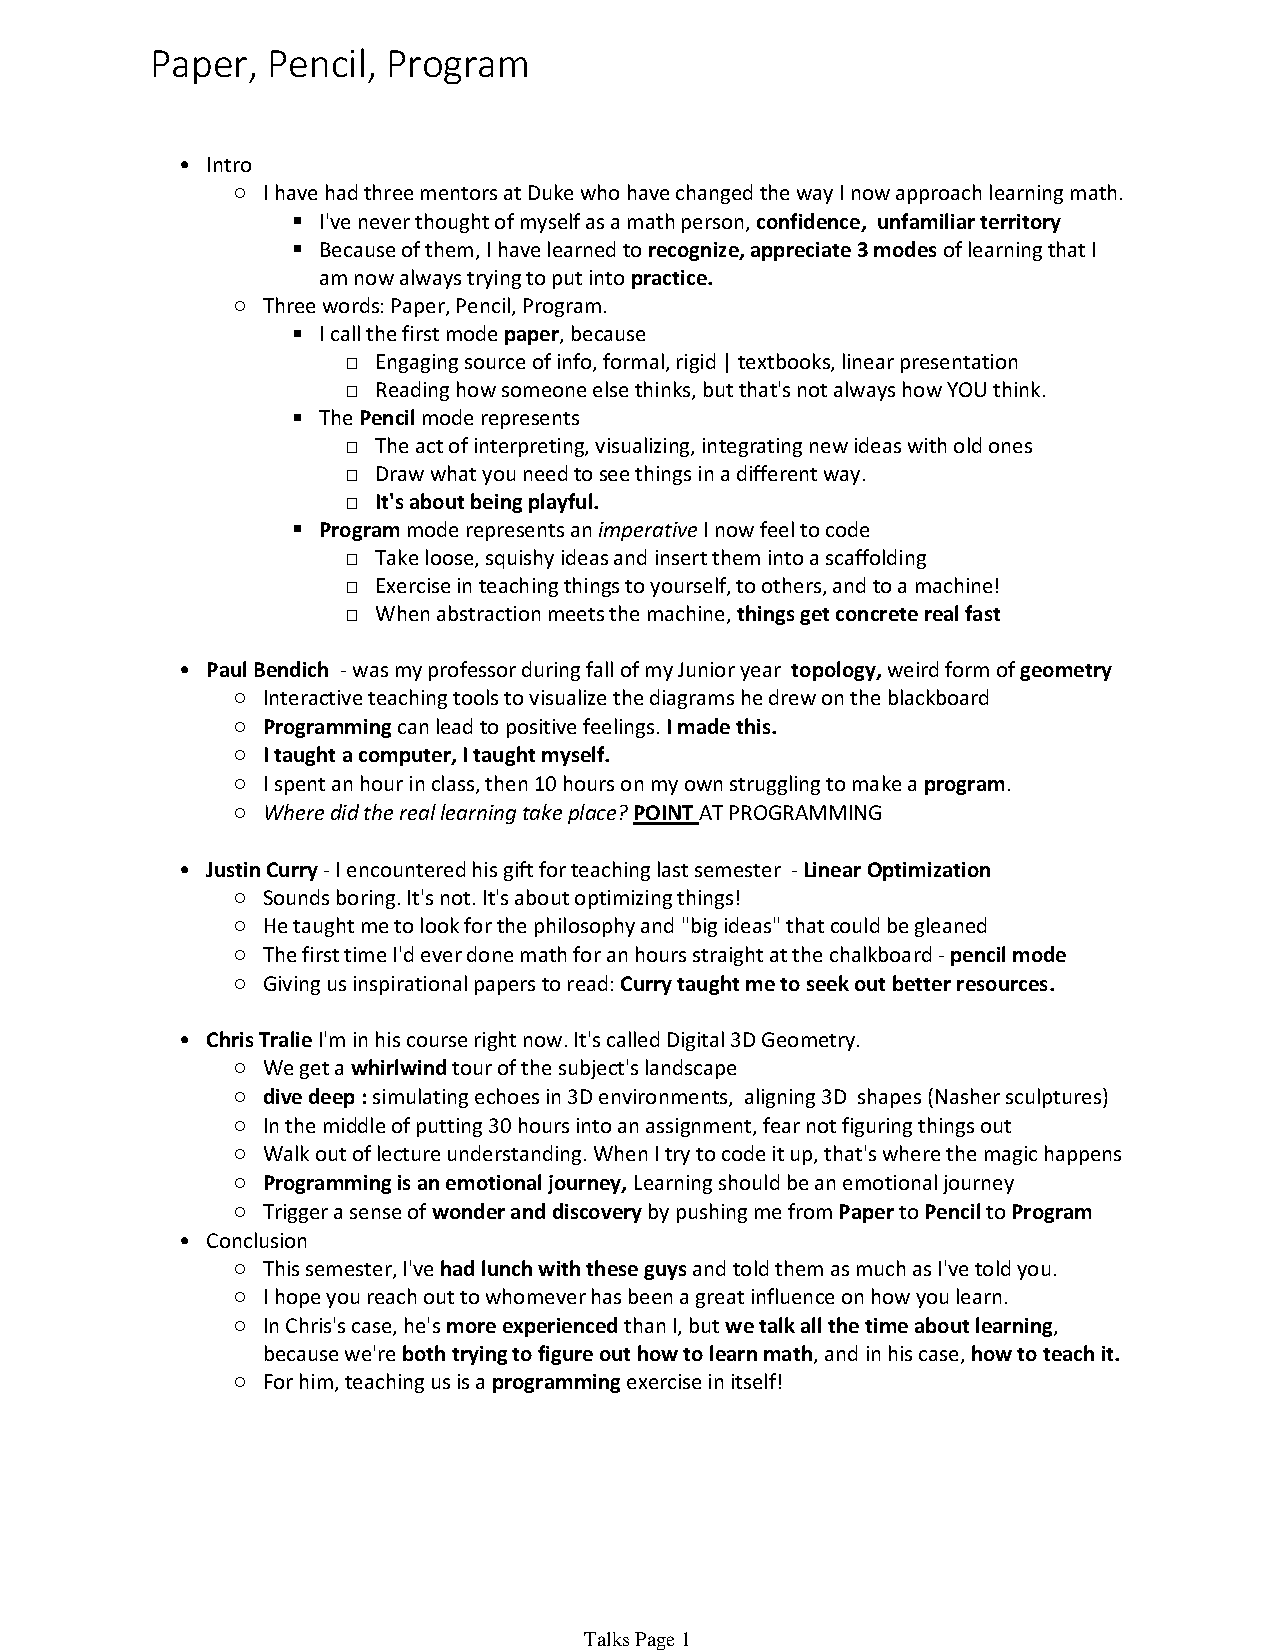
\includepdf[pages=-]{../external/paper-pencil-program.pdf}

\end{document}